\newpage
\part{Regression Analysis}
\section{Definition \& Terminology}
Regressions identify \textbf{relationship between dependent and independent variables}.
\begin{itemize}
	\item Association between dependent \& independent variables, 
	\item Impact of independent variables on dependent variables.
	\item Formulation of association/impact in functional form.
	\item Used for 
	\begin{itemize}
		\item descriptive analysis
		\item numerical prediction
		\item time series forcasting
	\end{itemize}
\end{itemize} 
\subsection*{Terminology}
\begin{itemize}
	\item \textbf{measurement tuples}: data streams  $(x_1,y_1), \dots, (x_n,y_n)$
	\item \textbf{predictor (independent variable, feature, regressor, covariate)}: $x_i$
	\item \textbf{response (dependent variable, outcome)}: $y_i$
	\item \textbf{regression function}: $\eta(x) = E(y|x)$
\end{itemize}






\section{Linear Regression}
\subsection{First Order Linear Model}

$$Y = \beta_0 + \beta_1 X + \varepsilon$$

\begin{itemize}
	\item Y: response variable (from measurement tuples)
	\item X: predictor variable (from measurement tuples)
	\item $\beta_0$: y-Axis intercept, \textbf{unknown, to be estimated} 
	\item $\beta_1$: slope, \textbf{unknown, to be estimated}
	\item $\varepsilon$: \textbf{residual}, random error 
\end{itemize}

\subsection{Multiple Linear Regression Model}
$$Y = \beta_0 + \beta_1 X_1 + \beta_2 X_2 + \dots + \beta_k X_k + \varepsilon$$
Formulation in \textbf{matrix form}:
$$\begin{bmatrix}
y_1 \\ y_2 \\ \vdots \\ y_m
\end{bmatrix} = \begin{bmatrix}
1 & X_11 &X_12 &\dots &X_1k \\
1 & X_21 &X_22 &\dots &X_2k \\
\vdots & \vdots &\vdots &\vdots &\vdots \\
1 & X_m1 &X_m2 &\dots &X_mk
\end{bmatrix} \begin{bmatrix}
\beta_0 \\ \beta_1 \\ \beta_2 \\ \vdots \\ \beta_k
\end{bmatrix} + \begin{bmatrix}
\varepsilon_1 \\ \varepsilon_2 \\ \vdots \\ \varepsilon_m
\end{bmatrix}$$
$$[m \times 1] = [m \times (k+1)] \cdot [(k+1) \times 1] + [m \times 1]$$

\textbf{OLS Estimator} for multiple linear regression model: minimize the RSS
\begin{itemize}
	\item Model:
	\begin{align*}
		RSS  &= e^{T} e = (y - X\hat{\beta})^T (y - X\hat{\beta}) \rightarrow \min \\
		\rightarrow  &\frac{\partial RSS}{\partial \beta} = -2X^Ty + 2X^TX\beta= 0
	\end{align*}
	
	\item Solution:
	\begin{align*}
		\hat{\beta} &= (X^TX)^{-1}X^Ty \\ \ \\
		\hat{y} &= X(X^TX)^{-1}X^Ty
	\end{align*}
	
	\item Projection: minimizing RSS $\rightarrow \vec{e}$ is orthogonal to the subspace spanned by all independent variables
	\begin{figure}[H]
		\centering
		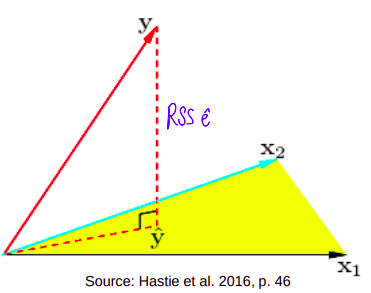
\includegraphics[width=0.4\textwidth]{projection.png}
	\end{figure}
\end{itemize}

\subsection{Estimation of Coefficients: Ordinary Least Square Estimator}
\begin{itemize}
	\item input: data streams $(x_i, y_i)$
		  
		  model: linear regression $Y = \beta_0 + \beta_1 X + \varepsilon$ 
		  
		  output: $\hat{\beta}_0$, $\hat{\beta}_1$
	\item Goal of OLS estimator: \textbf{minimize the sum of squared residuals (RSS) } 
	
	Outlier will have larger value input when residual squared.
	$$\hat{y} = \hat{\beta}_0 + \hat{\beta}_1 x$$
	$$\min{\Sigma_i e_i^2} = \min{\Sigma_i (y - \hat{y})^2} = \min{\Sigma_i (y - (\hat{\beta}_0 + \hat{\beta}_1 x))^2} $$
	
\end{itemize}
\subsection{Quality Metrics of the Model}
To measure how well the model fits the data, you can analyze the quality model-wise or coefficient-wise.
\begin{itemize}
	\item Model-wise: 
	\begin{itemize}
		\item Residual Sum of Squares (RSS)
		\item Total Sum of Squares (TSS)
		\item $R^2$
	\end{itemize}
	\item Coefficient-wise:
	\begin{itemize}
		\item Significance-Test on each coefficient in the model
	\end{itemize}
\end{itemize}
\subsubsection{Residual Sum of Squares (RSS)}
An \textbf{unbiased} estimator of RSS of the population is given by 
$$RSS = \Sigma_{i=1}^{n} (y_i - \hat{y}_i)^2$$
\begin{itemize}
	\item RSS = 0: the model fits 100\% of the data
	\item RSS $\neq$ 0: distance between true $y$ and $\hat{y}$ : residual $e$
	\item RSS $\downarrow$, model-fit quality $\uparrow$
\end{itemize}
\subsubsection{Mean Squared Error (MSE)}
$$MSE = \frac{RSS}{N}$$
\subsubsection{Root Mean Squared Error (RMSE)}
$$RMSE = \sqrt{MSE}$$
\subsubsection{Total Sum of Squares (TSS)}
\textbf{Total Sum of Squares(TSS)} is the sum of Explained Sum of Squares(ESS) and Residual Sum of Squares(RSS).
\begin{align*}
	\Sigma (y - \bar{y})^2 &= \Sigma (\hat{y} - \bar{y})^2 + \Sigma (y - \hat{y})^2 \\
	TSS &= ESS + RSS
\end{align*}
\subsubsection{$\mathbf{R^2}$}
$R^2$ measures the proportion of the variation in y that is explained by the variation in x. $\rightarrow$ the \textbf{proportion of Explained Sum of Squares(ESS).}
$$R^2 = \frac{TSS - RSS}{TSS} = 1 - \frac{RSS}{TSS} = \frac{ESS}{TSS}$$ 
\begin{itemize}
	\item range of $R^2$: [0,1]
	\begin{itemize}
		\item $R^2 = 0$: ESS = 0, RSS = $\infty$. No linear relationship between x and y.
		\item $R^2 = 1$: ESS = TSS, RSS = 0. Perfect match between x and y.
	\end{itemize}
\end{itemize}

\subsubsection{Significance Test of the coefficients: T-Test}
\begin{itemize}
	\item Test the significance of the coefficients in alternative hypothesis($H_1$):
	$$H_0: \beta_1 = 0$$
	$$H_1: \beta_1 \neq 0$$
	\item Distribution: T-Distribution
	\item Degree of Freedom: if \textbf{error variable} is \textbf{normally distributed}, then $$df = n - 2 $$
	\item test statistic:
	\large{$$t = \frac{\hat{\beta}_1 - 0}{SE(\hat{\beta}_1)} = \dfrac{\hat{\beta}_1}{\sqrt{\frac{RSS}{\Sigma_{i=1}^n (x_i - \bar{x})^2} \cdot \frac{1}{n-2}}}$$}
	\item Conclusion: 
	
	two-sided test, reject $H_0$, if $|t| > t^c_{1-\frac{\alpha}{2}}$ or $p < \alpha$
	
\end{itemize}
\subsubsection{Other Metrics}
\begin{itemize}
	\item Adjusted $R^2$: allows models \textbf{with different number of variables} to be compared
	\item F-statistic: indicates linear relationship between y and \textbf{at least one} of the xs
	\item T-test of each partial regression coefficient: significance of a single coefficient while controlling others
\end{itemize}



\subsection{Model Specification}
The process of developing a regression model. It's a repeated process. You need to try different combinations or test the significance of variables to find an optimal regression model.

\begin{itemize}
	\item selection of an appropriate functional form (linear, quadratic, log-linear, interaction terms, etc.)
	\item choosing which variables to include (might include irrelevant or omit relevant variables)
\end{itemize}

\subsubsection{Functional Form of Linear Model} 
\begin{itemize}
	\item standard normal linear model(first-order/multiple)
	\item nominal variables(categorical): 0 or 1
	\item quadratic models: $y = \beta_0 + \beta_1 x_1 + \beta_2 x_2^2 \rightarrow z_2 = x_2^2$ 
	\item interaction terms: $y = \beta_0 + \beta_1 x_1 + \beta_2 x_1x_2 \rightarrow z_2 = x_1x_2$
	\item exponential terms into logarithm terms: $y = \alpha x^{\beta}\varepsilon \rightarrow \ln(y) = \ln(\alpha) + \beta\ln{x} + \ln(\varepsilon)$
\end{itemize}

\subsubsection{Choosing Variables to Include}
\begin{itemize}
	\item Idea: The initial model might include large set of irrelevant variables or omit some relevant variables. 
	\item Goal: find an optimal combination that explains variation in Y with \textbf{a small and meaningful predictors Xs} $\rightarrow$ feature selection
	\item Methods:
	\begin{itemize}
		\item \textbf{Best Subset}: 
		
		Test \textbf{all combinations} ($2^n$) and find out best subset 
		\item \textbf{Backward Elimination}: (top-down)
		
		Start with\textbf{ full model with all variables}, test the significance(t-Test) of the variables.
		
		Consider the predictor with lowest t-statistic/highest p-value: remove the variable if $p > \alpha$ (can't reject $H_0$)  
		\item \textbf{Forward Selection}: (buttom-up)
		
		Start with \textbf{only one variable}, test the significance(t-Test) of the variable.
		
		Only consider the variable with highest t-statistic/lowest p-value: add the variable if $p < \alpha$ (reject $H_0$)
		\item \textbf{Stepwise Regression}: combination of forward/backward selection.
	\end{itemize}
\end{itemize}
 
\subsection{Model Interpretation}
Result of a model fitting can be retrieved by ''summary(model)''
\begin{itemize}
	\item Hypothesis:
	\begin{itemize}
		\item Parameters: 
		
		$H_0$: $\beta_i = 0$
		
		$H_1$: $\beta_i \neq 0$
		\item Whole Model: 
		$H_0$: All predictors are not able to explain the model.
		
		$H_1$: The whole model is statistically significant. 		 
	\end{itemize}
	\item Conclusion: 
	
	for an $\alpha = 0.05$ level, $p > \alpha, \rightarrow$ cannot reject $H_0$, the parameter x is not significant from 0. 
\end{itemize}
\begin{figure}[H]
	\centering
	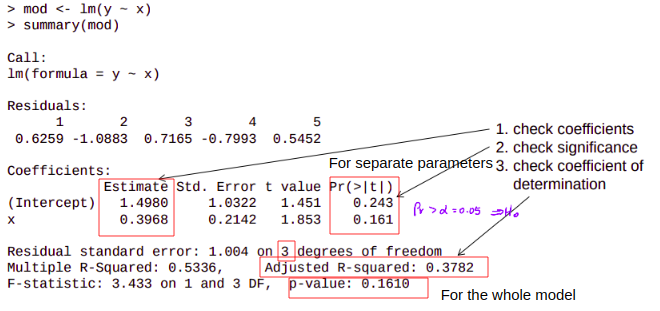
\includegraphics[width=0.9\textwidth]{lm_R.png}
\end{figure}	

\subsubsection*{Interpretation}
\begin{itemize}
	\item \textbf{predictors, intercepts -- coefficient \& p-value}: 
	\begin{itemize}
		\item Significance: significant? at a significance level of $\alpha$ = ?
		\item $\beta_0$: intercept, the value when all predictors are 0.
		\item $\beta_i$: slope, coefficient positive/negative influence of predictors on response? 
		\item \textbf{Transformed} predictors/response
	\end{itemize} 
	\item \textbf{whole model -- F-statistic \& p-value}: significant? at a significance level of $\alpha$ = ?
	\item \textbf{Explanatory power of the model -- Adjusted $R^2$}: high/low? why?
	
\end{itemize}


